\documentclass[onecolumn]{preport}
\usepackage[dvipdfmx]{color}
\usepackage[dvipdfmx]{graphicx}
\usepackage[subrefformat=parens]{subcaption}
\usepackage{listings}
\usepackage{color}
\usepackage{here}
\usepackage{url}
\graphicspath{{figs/}}
\title{クラウド基盤ソフトウェア課題レポート2}
\author{480206515 知能機械情報学専攻 河村洋一郎}

\begin{document}

\pagestyle{empty}
\maketitle
\thispagestyle{empty}
\sloppy

\section{実験設定}
\subsection{実験に用いた計算機}
実験は研究室のPCで行った.計算機のスペックは以下.
\begin{table}[htb]
  \begin{tabular}{c|l} \hline
    CPU & Intel(R) Core(TM) i9-7980XE CPU @ 2.60GHz \\ \hline
    メモリ & 128GB DDR4 \\ \hline
  \end{tabular}
\end{table}

\section{実験}
JavaScrpitでフィボナッチ数を計算するプログラムを実行し,実行速度を比較した.
作成したコードは~\cite{myrepo}に記載した.また,同様の実験を16回繰り返した.
\begin{enumerate}
\item $Fib(1000)$を求める計算を50回繰り返す
\item $Fib(n)$を1から1000まで求める計算
\end{enumerate}
実験1回(1, 2を実行)あたりの結果は\figref{fib}のようになる.
$\vspace{0.5cm}$

$\hspace{0.5cm}$ $Fib(1000)$を求める計算を50回繰り返す処理$\hspace{3cm}$ $Fib(n)$を1から1000まで求める処理
\begin{figure}[H]
  \begin{center}
    \begin{minipage}{0.99\columnwidth}   
      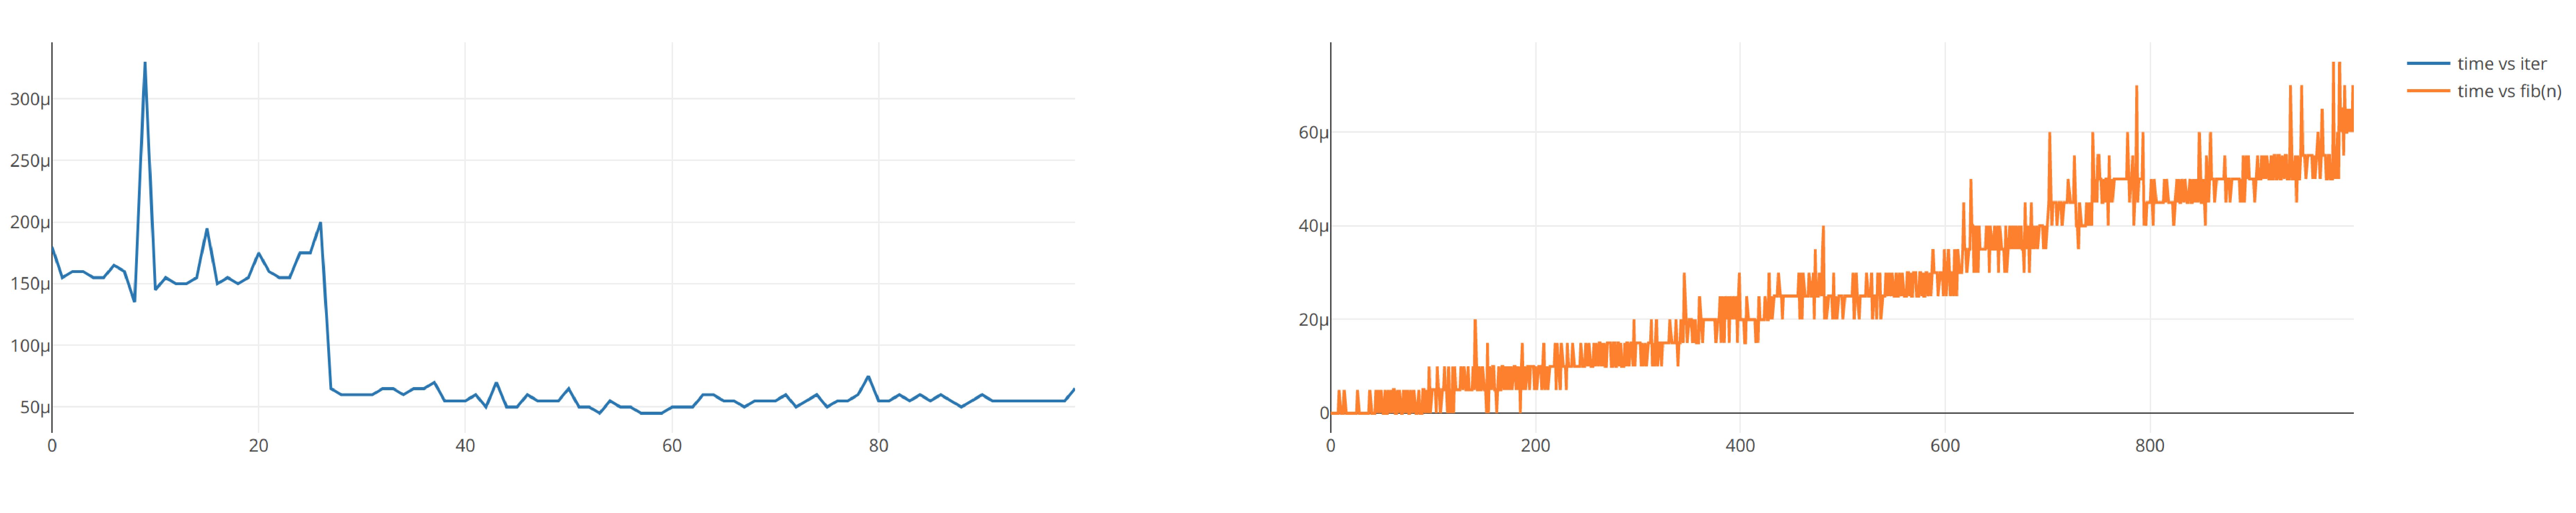
\includegraphics[width=\columnwidth]{figs/result.pdf}
      \caption{結果の一例}
      \label{figure:fib}
    \end{minipage}
  \end{center}
\end{figure}



\section{結論,考察}
16回実験を行った結果を\figref{16}に示す.まず,実験1( $Fib(1000)$を求める計算を50回繰り返す処理, 青色)について、全体の傾向として、ある回数までは時間がかかり、途中から極端に処理時間が短くなることがわかる。全体的にスパイク的に処理速度が伸びることがあることもわかる。

一方で、処理時間が短くなるタイミングについては、毎回一定ではなく、(c)のように30回程度の繰り返しで処理速度が短くなる場合もあれば、(p)のように10回程度で処理速度が短くなる場合もある。

さらに興味深い挙動としては、(a)のように、スパイクがある回数ほかの試行に比べて多い場合や、(i)のように一度処理時間が短くなったあとで、処理時間が再度長くなる試行が挙げられる。特に(i)は、コンパイラが簡易的なコンパイルにダイナミックに変更する(普段とは逆方向)にあることを意味し、現状自分ではなぜこのようなこ
とが起きるのかわからなかった。

実験2($Fib(n)$を1から1000まで求める計算, オレンジ色)では、実験1と同様にスパイクがあるが、実験1ではスパイクしても処理速度が2倍程度に上がるだけだったのに対し実験2では、スパイクすると40〜50倍程度に上がっている。


\begin{figure}[H]
  \begin{center}
    \begin{minipage}{0.23\columnwidth}   
      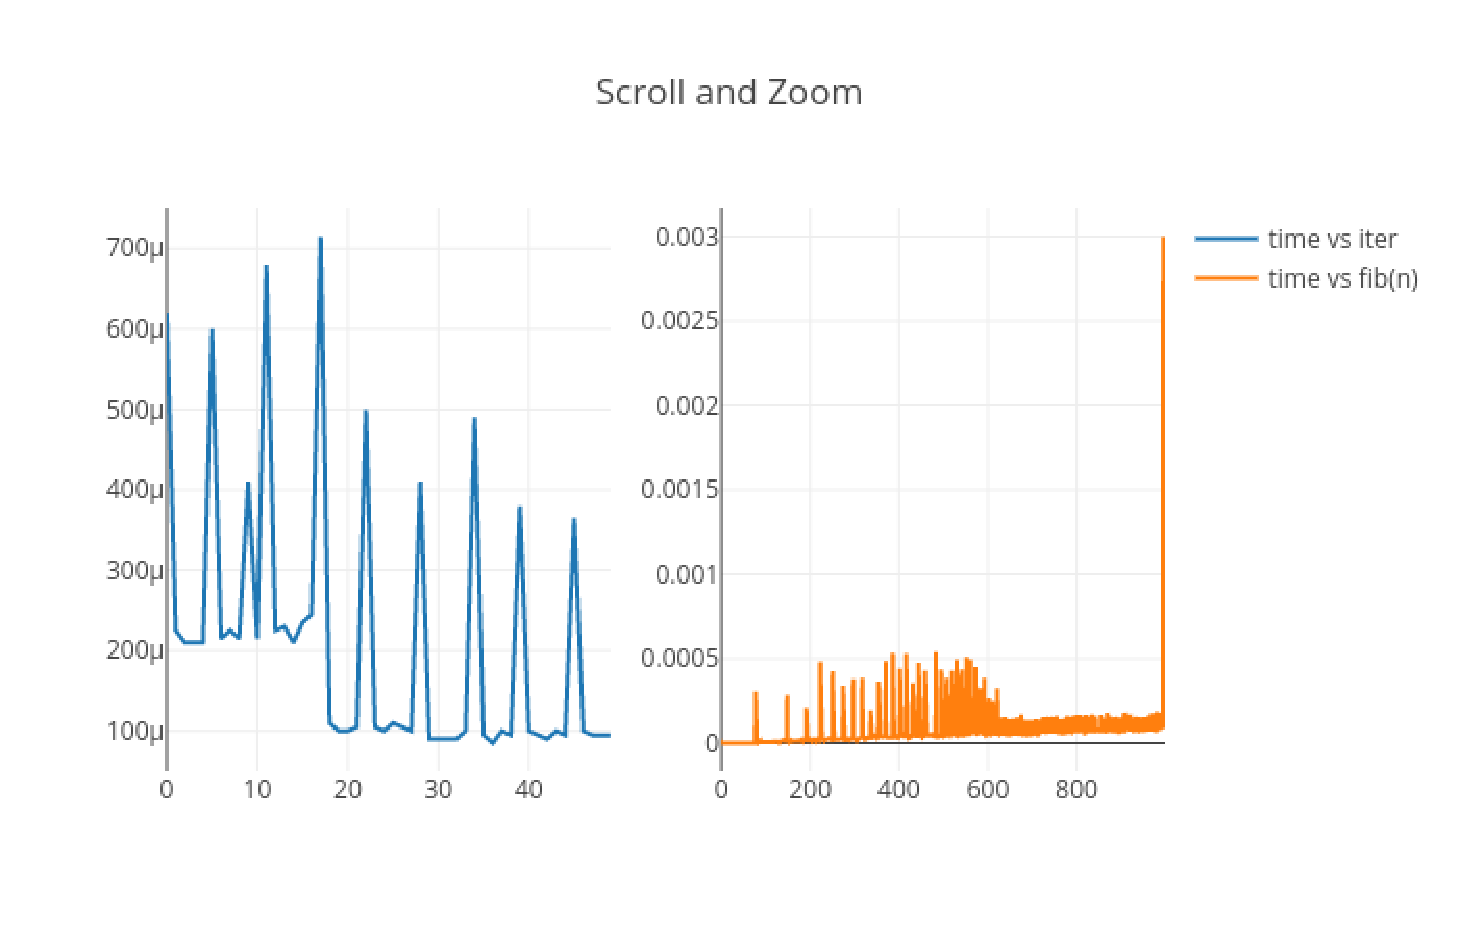
\includegraphics[width=\columnwidth]{figs/newplot1.pdf}
      \subcaption{}
    \end{minipage}
    \begin{minipage}{0.23\columnwidth}   
      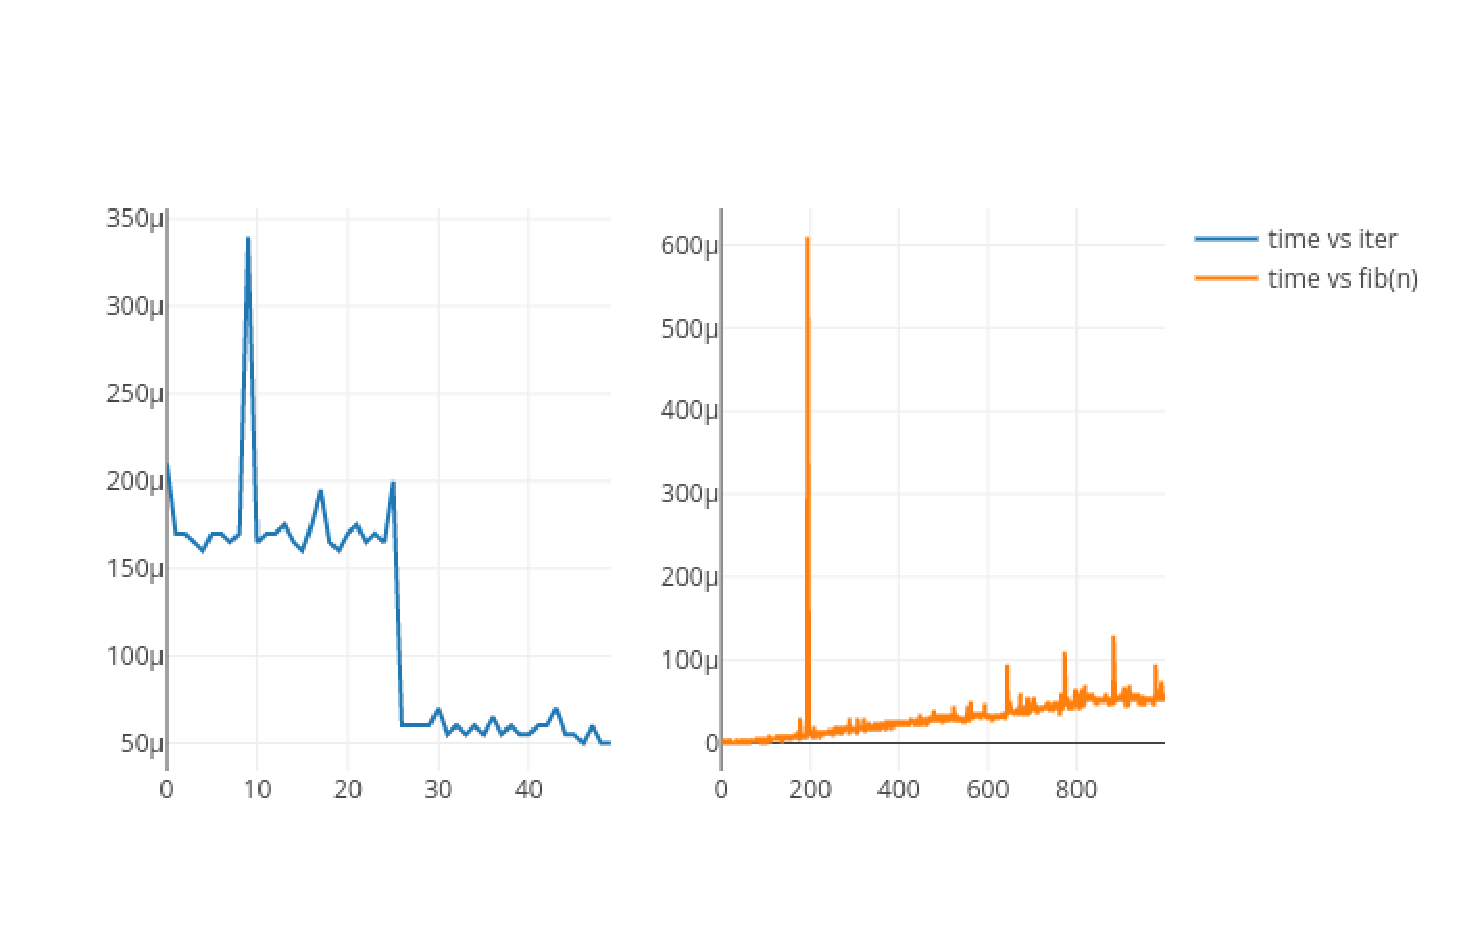
\includegraphics[width=\columnwidth]{figs/newplot2.pdf}
      \subcaption{}
    \end{minipage}
    \begin{minipage}{0.23\columnwidth}   
      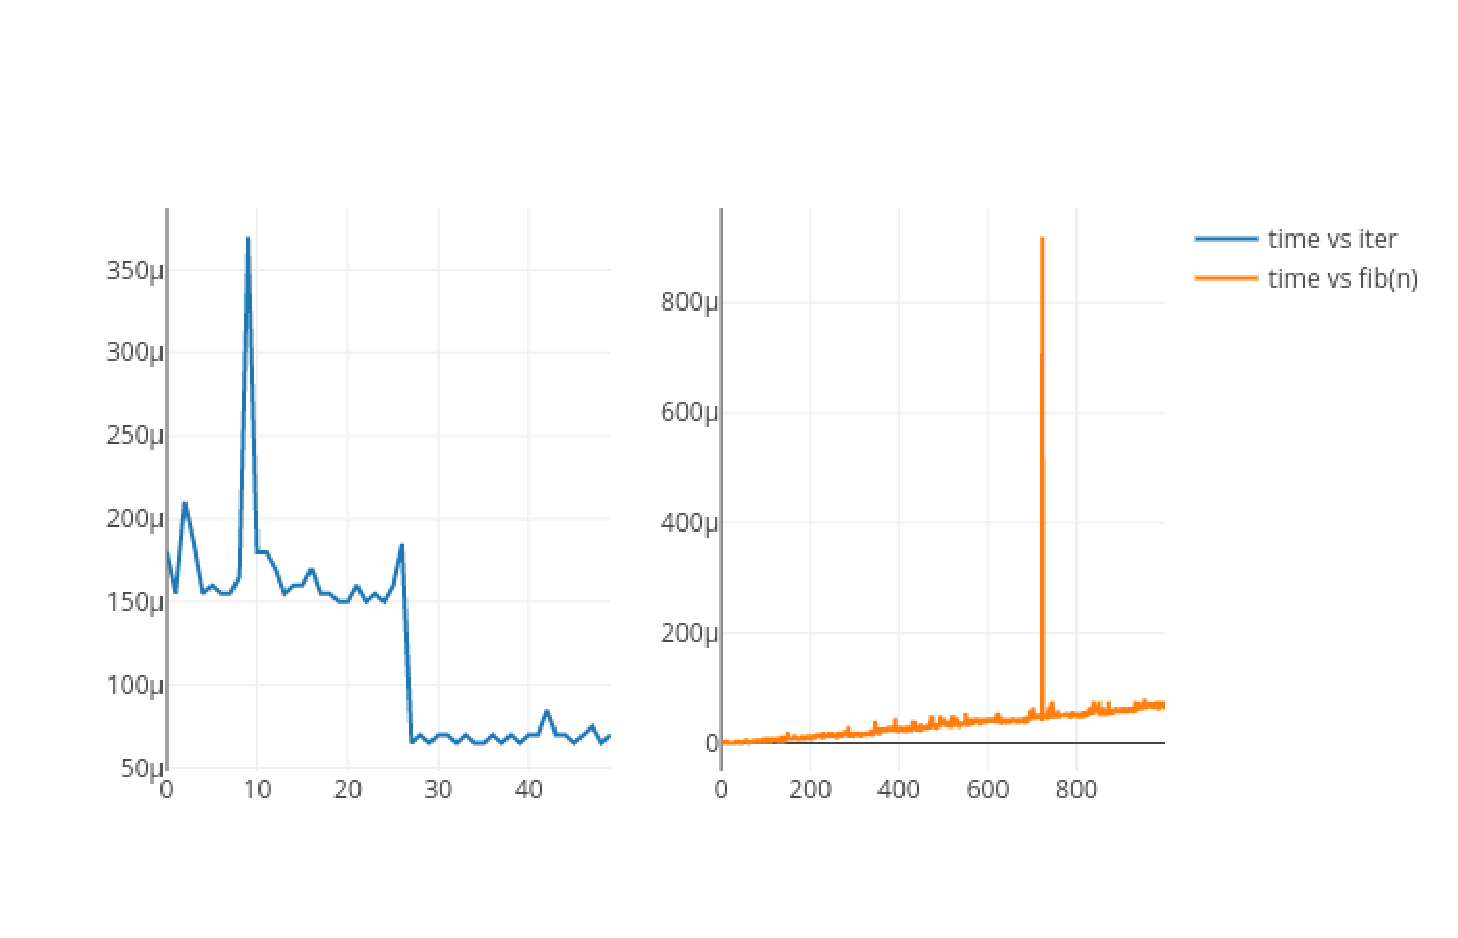
\includegraphics[width=\columnwidth]{figs/newplot3.pdf}
      \subcaption{}
    \end{minipage}
    \begin{minipage}{0.23\columnwidth}   
      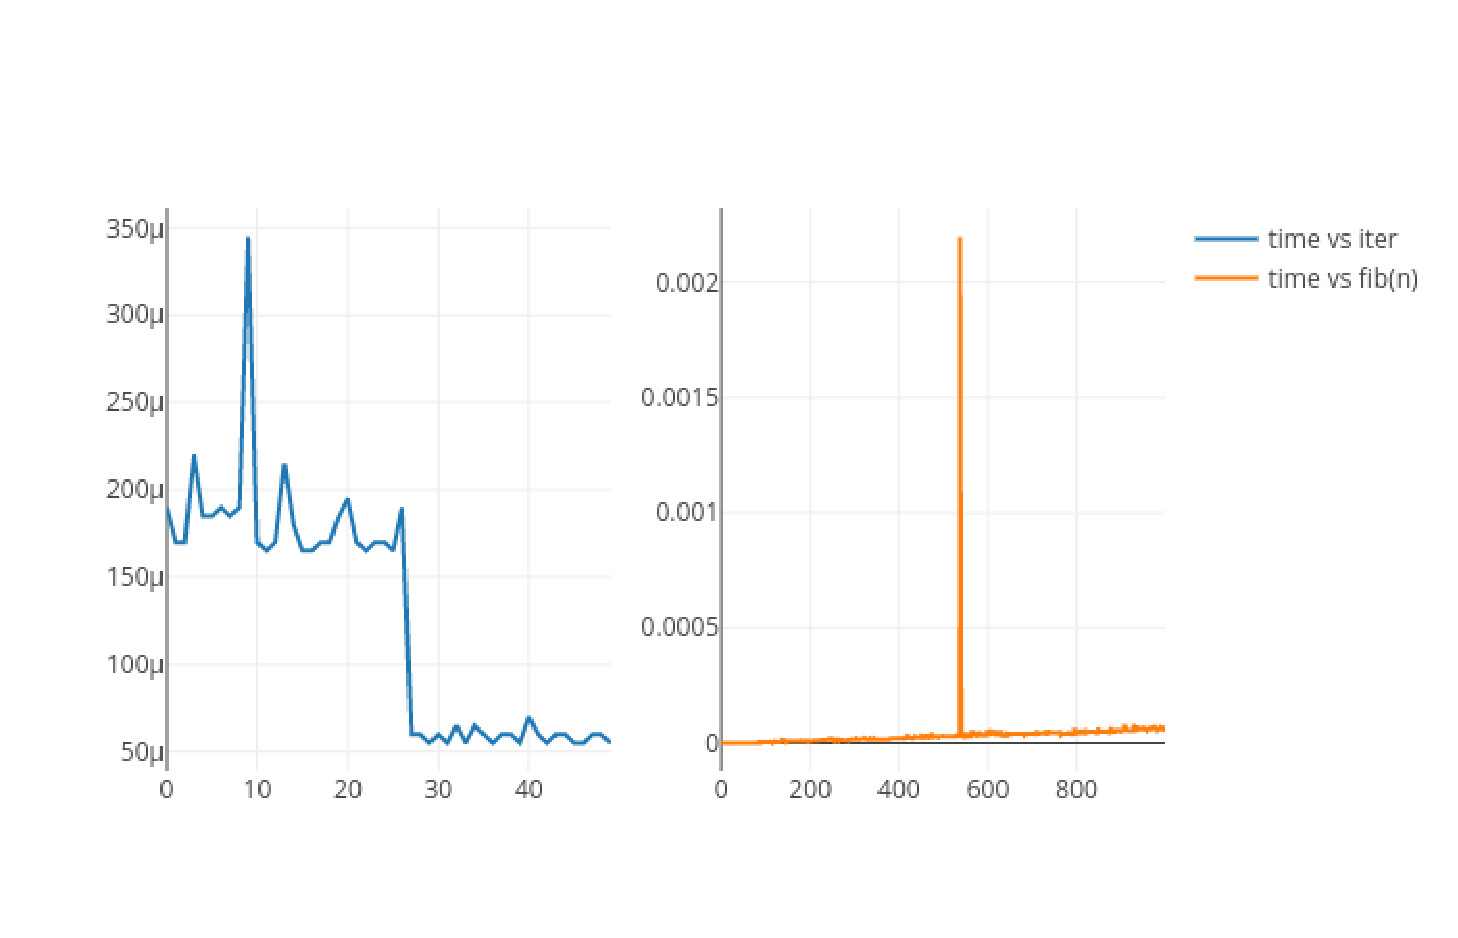
\includegraphics[width=\columnwidth]{figs/newplot4.pdf}
      \subcaption{}
    \end{minipage}
    \begin{minipage}{0.23\columnwidth}   
      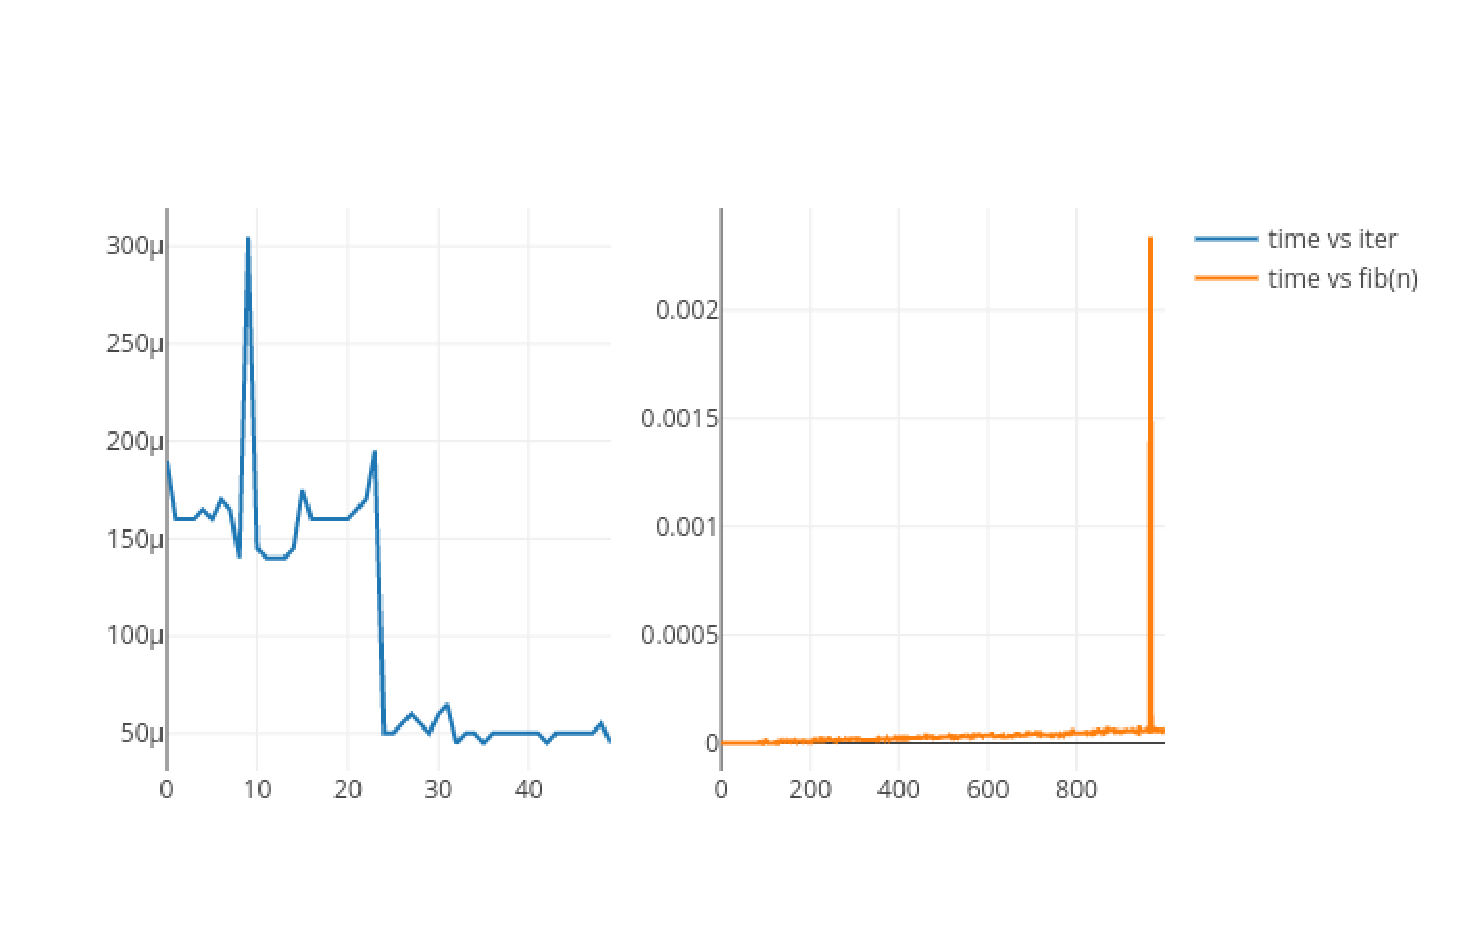
\includegraphics[width=\columnwidth]{figs/newplot5.pdf}
      \subcaption{}
    \end{minipage}
    \begin{minipage}{0.23\columnwidth}   
      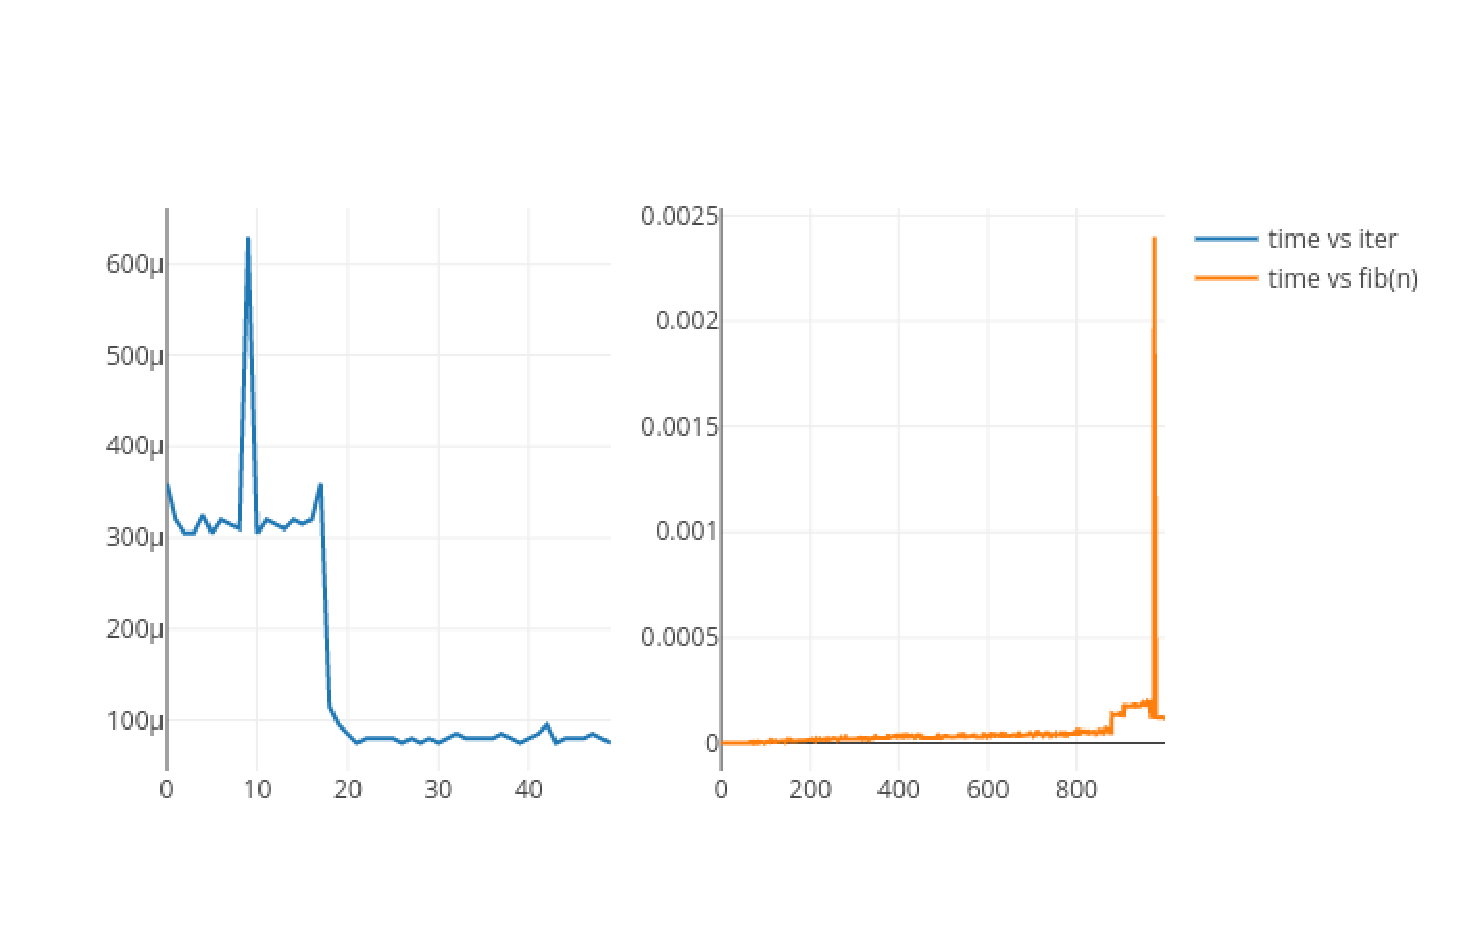
\includegraphics[width=\columnwidth]{figs/newplot6.pdf}
      \subcaption{}
    \end{minipage}
    \begin{minipage}{0.23\columnwidth}   
      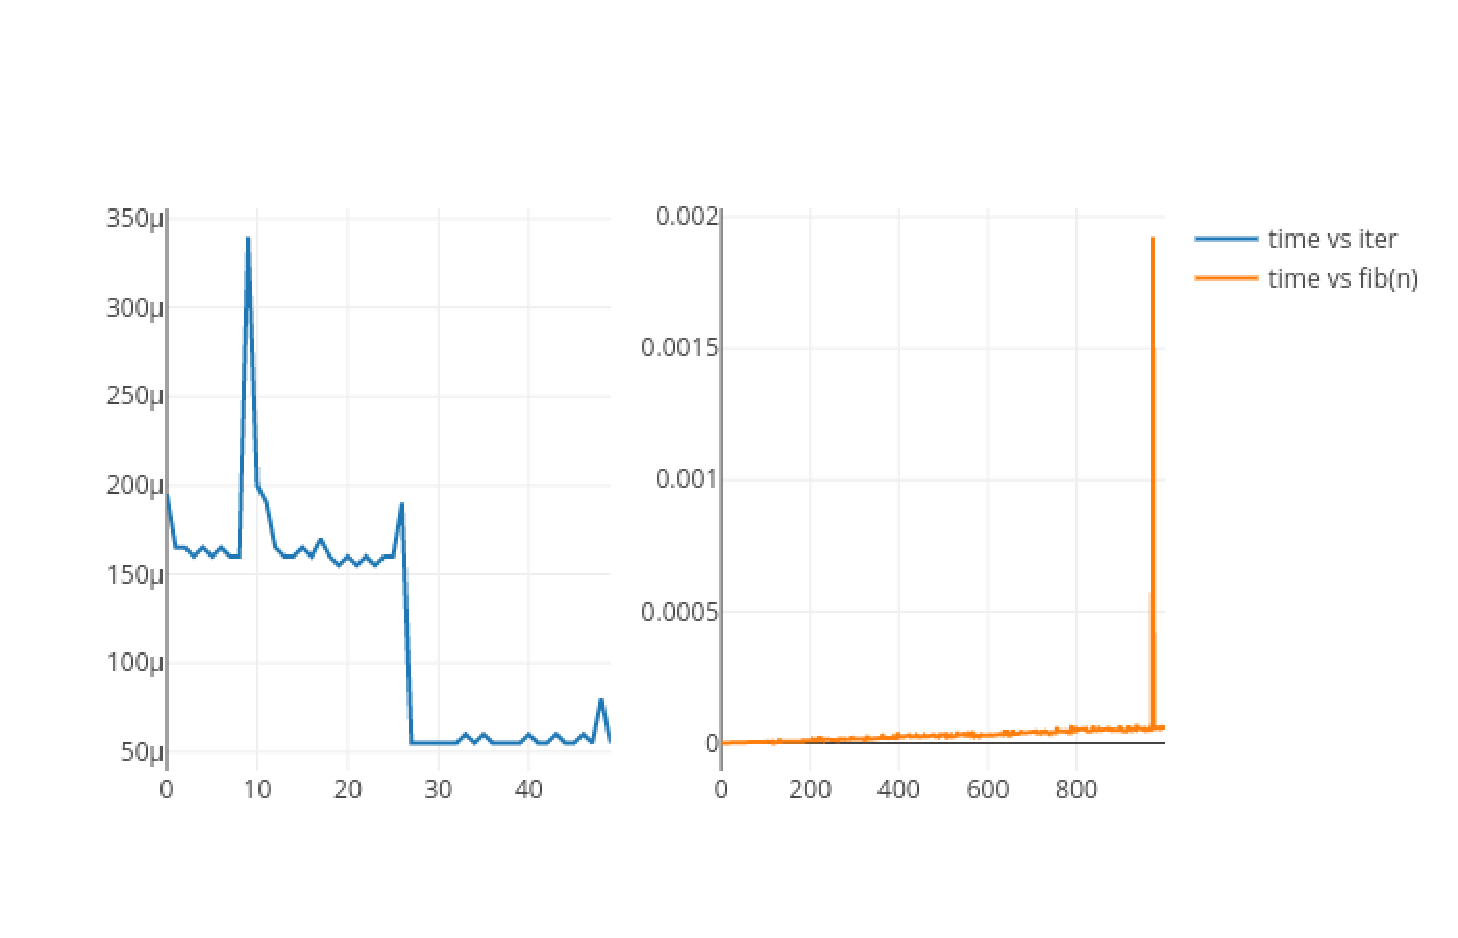
\includegraphics[width=\columnwidth]{figs/newplot7.pdf}
      \subcaption{}
    \end{minipage}
    \begin{minipage}{0.23\columnwidth}   
      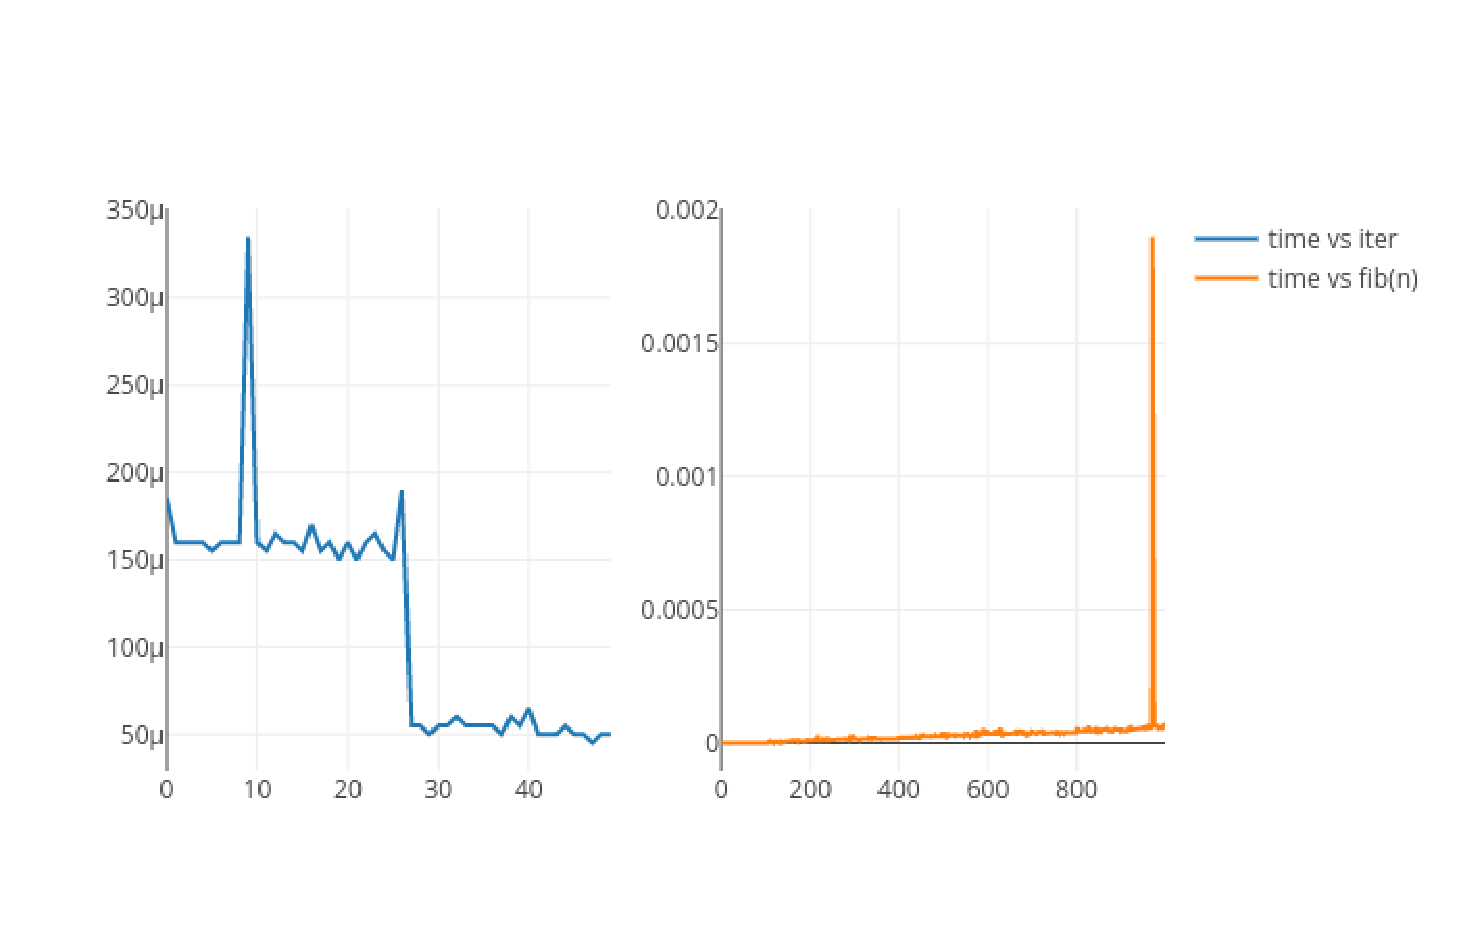
\includegraphics[width=\columnwidth]{figs/newplot8.pdf}
      \subcaption{}
    \end{minipage}
    \begin{minipage}{0.23\columnwidth}   
      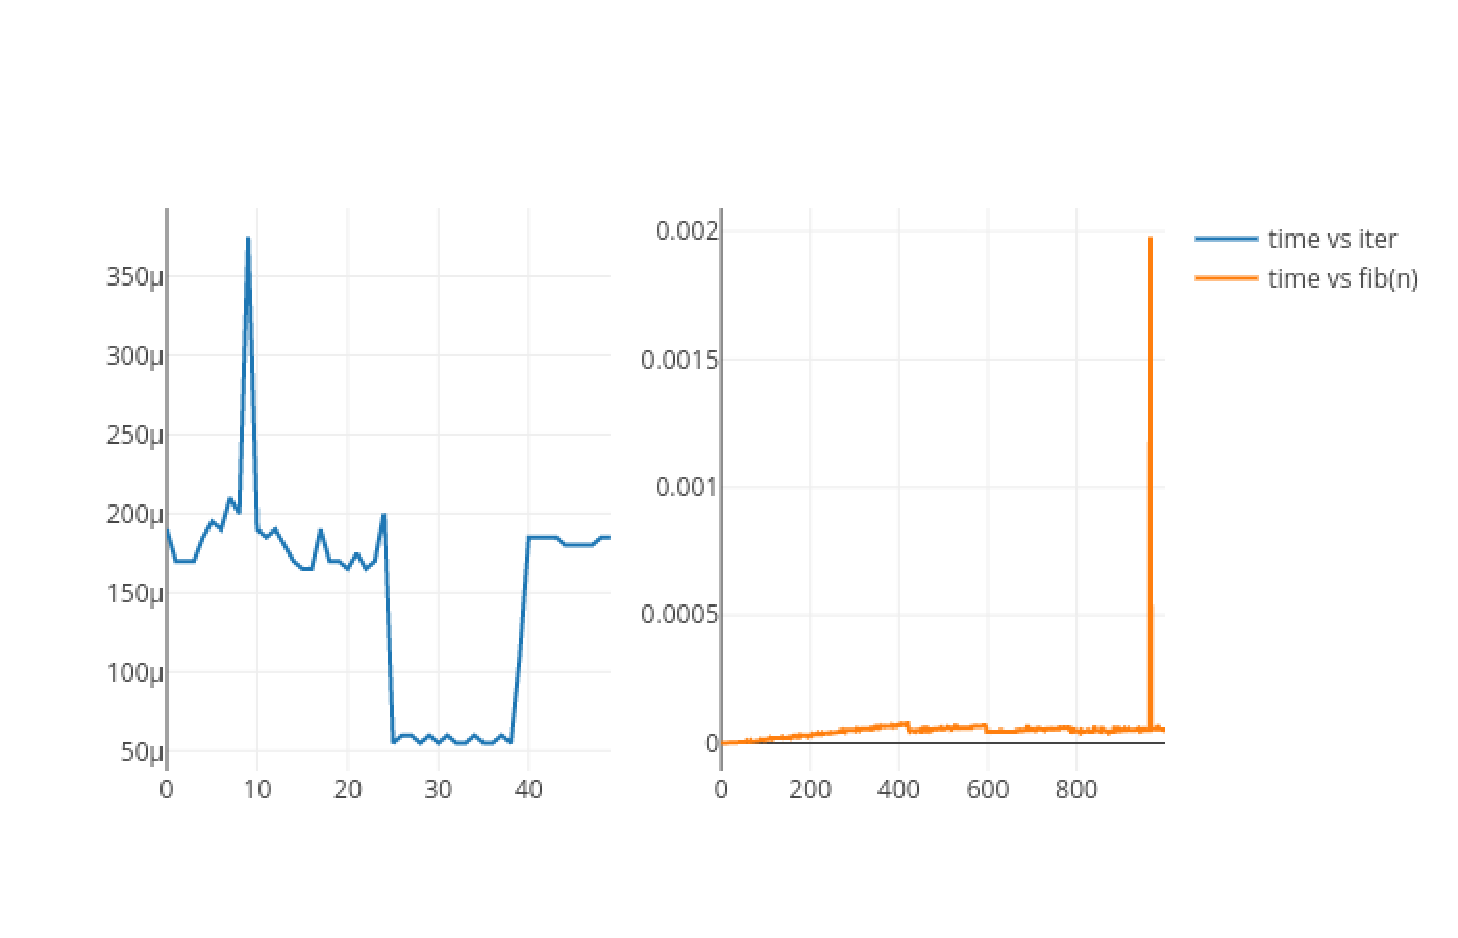
\includegraphics[width=\columnwidth]{figs/newplot9.pdf}
      \subcaption{}
    \end{minipage}
    \begin{minipage}{0.23\columnwidth}   
      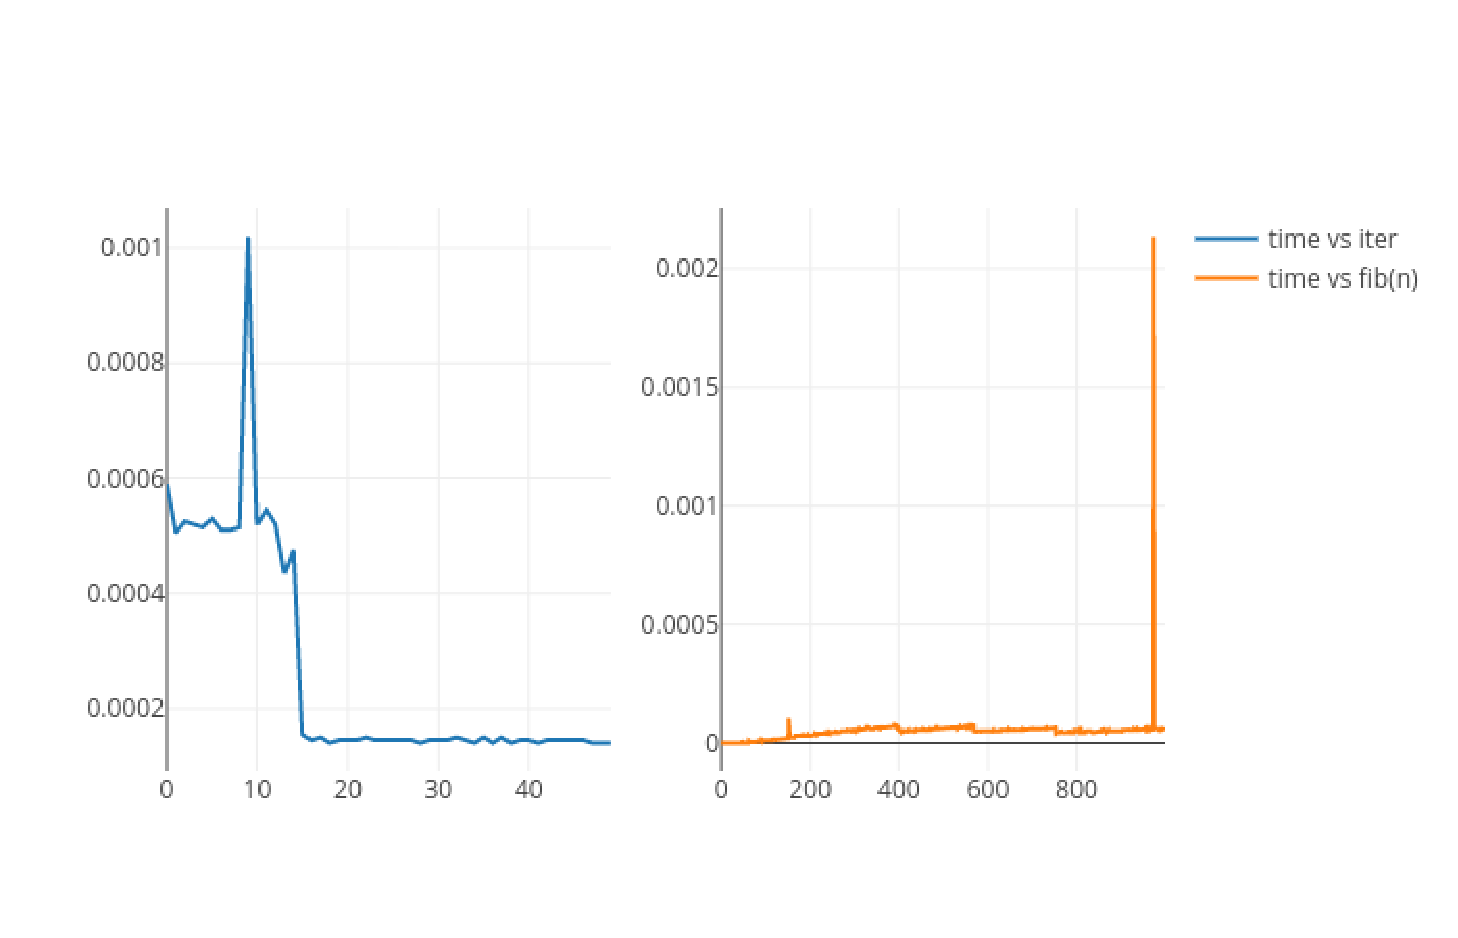
\includegraphics[width=\columnwidth]{figs/newplot10.pdf}
      \subcaption{}
    \end{minipage}
    \begin{minipage}{0.23\columnwidth}   
      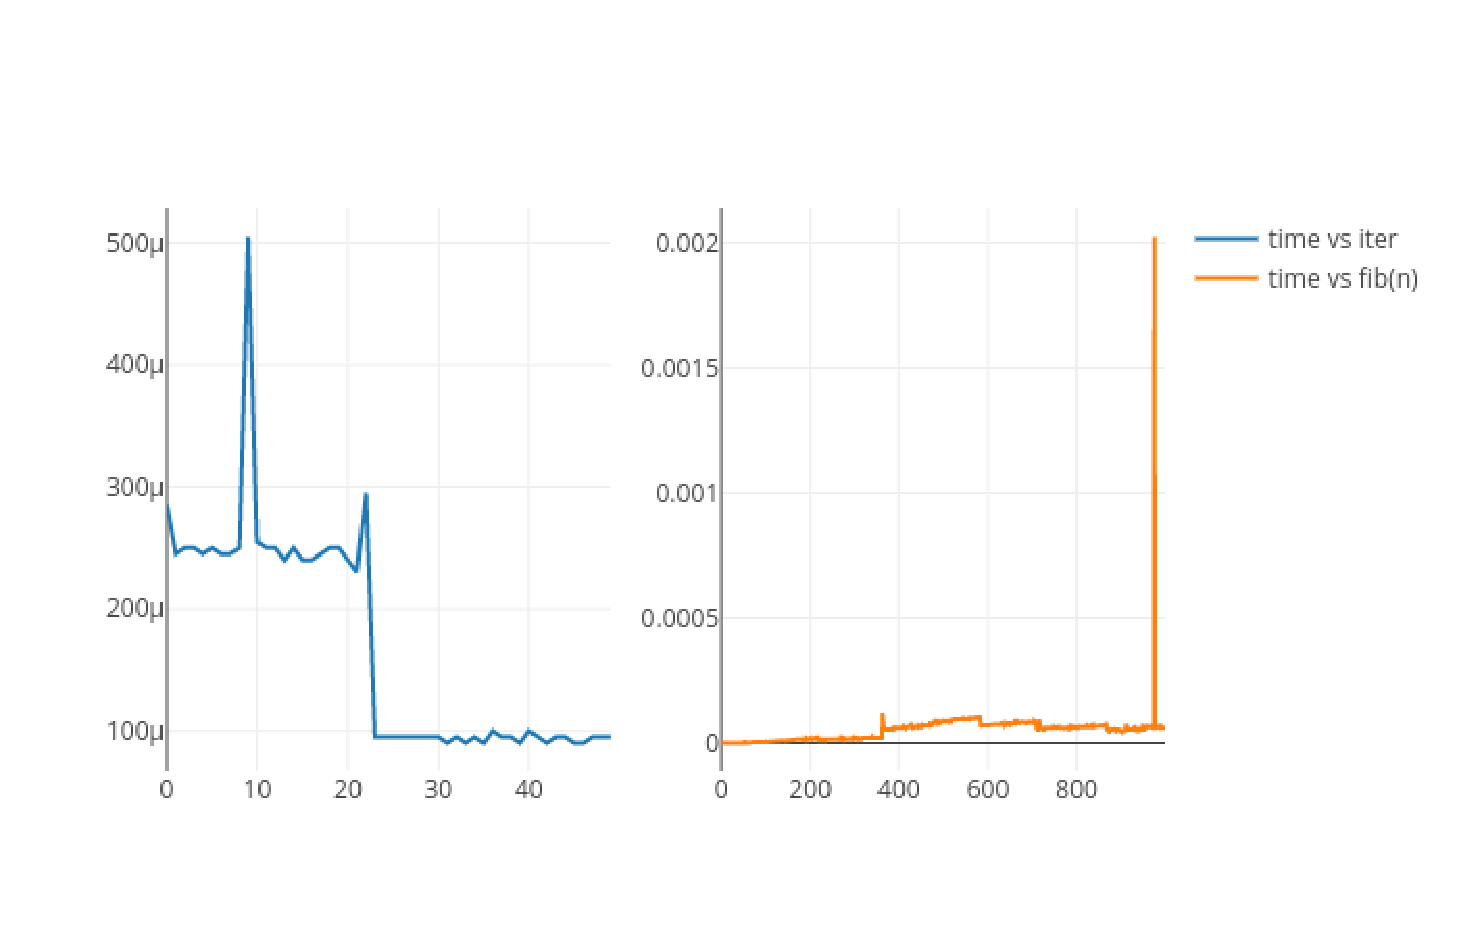
\includegraphics[width=\columnwidth]{figs/newplot11.pdf}
      \subcaption{}
    \end{minipage}
    \begin{minipage}{0.23\columnwidth}   
      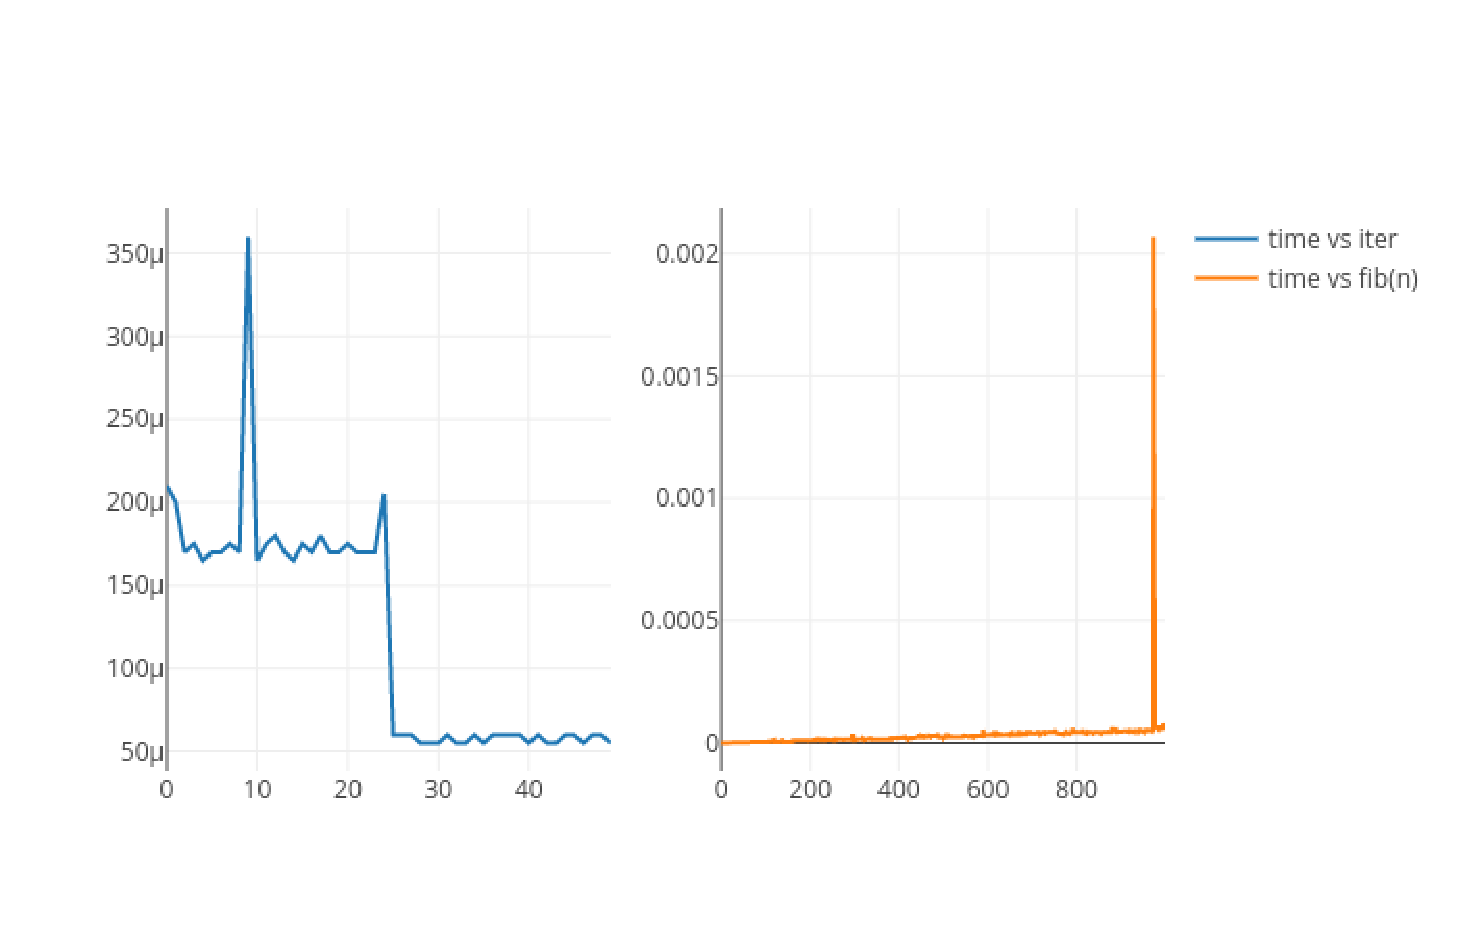
\includegraphics[width=\columnwidth]{figs/newplot12.pdf}
      \subcaption{}
    \end{minipage}
    \begin{minipage}{0.23\columnwidth}   
      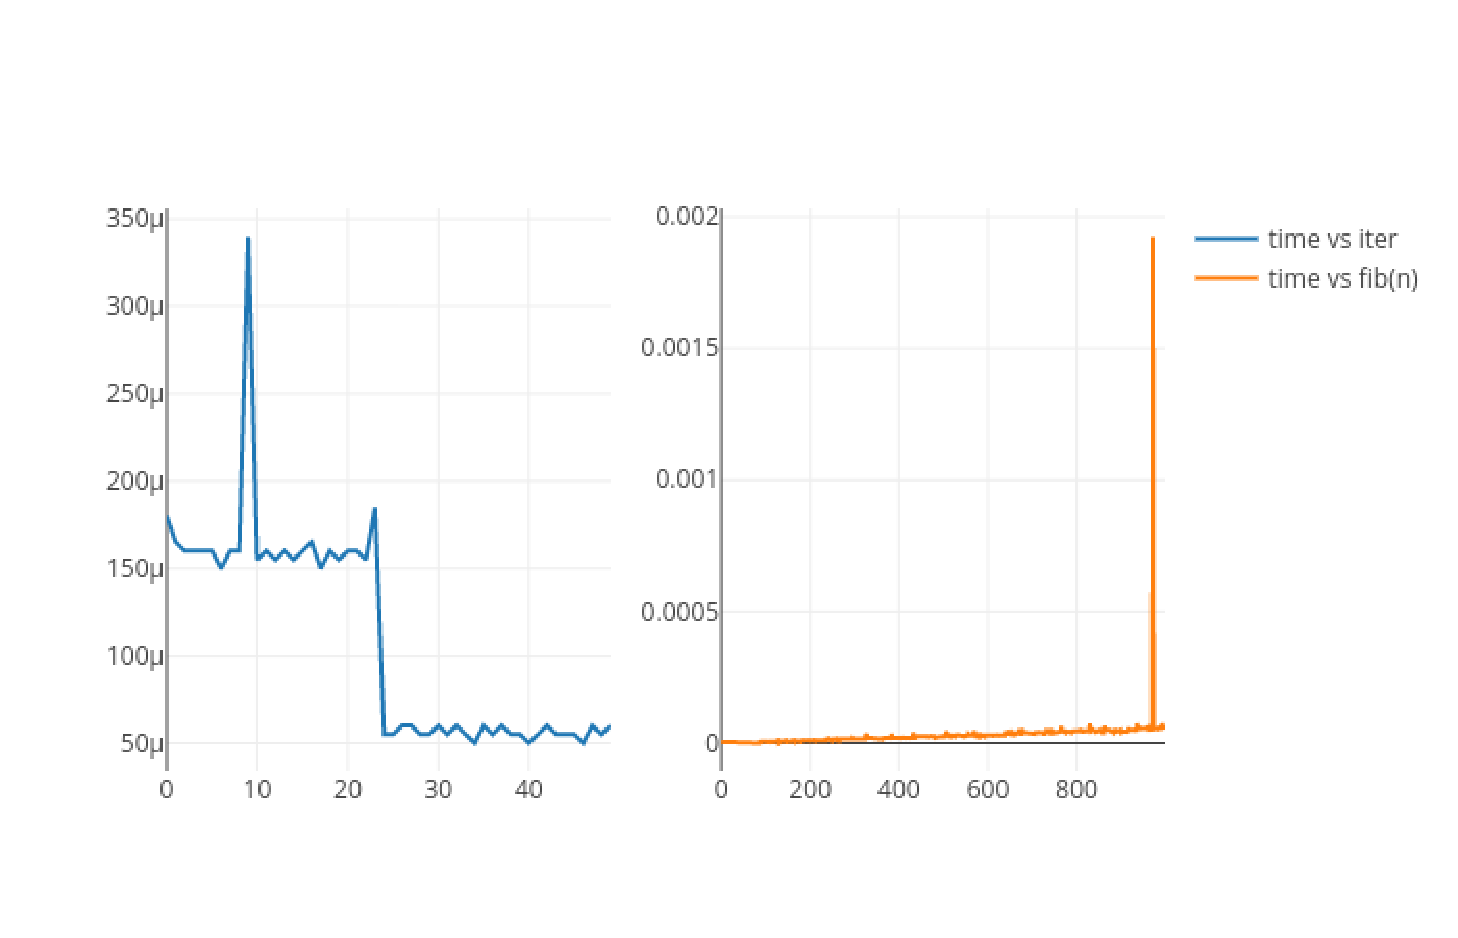
\includegraphics[width=\columnwidth]{figs/newplot13.pdf}
      \subcaption{}
    \end{minipage}
    \begin{minipage}{0.23\columnwidth}   
      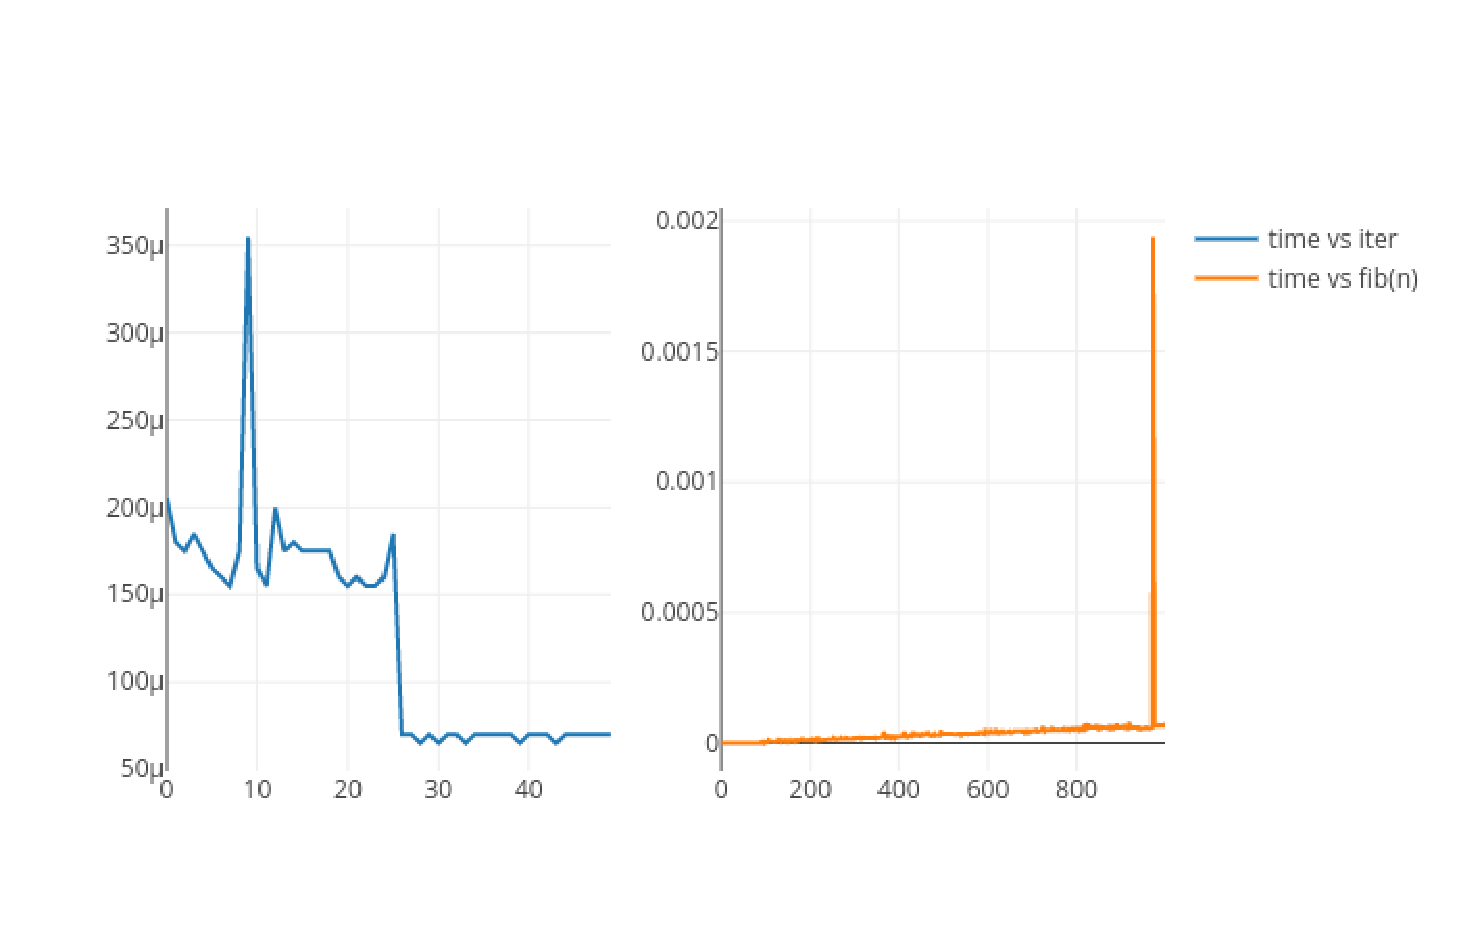
\includegraphics[width=\columnwidth]{figs/newplot14.pdf}
      \subcaption{}
    \end{minipage}
    \begin{minipage}{0.23\columnwidth}   
      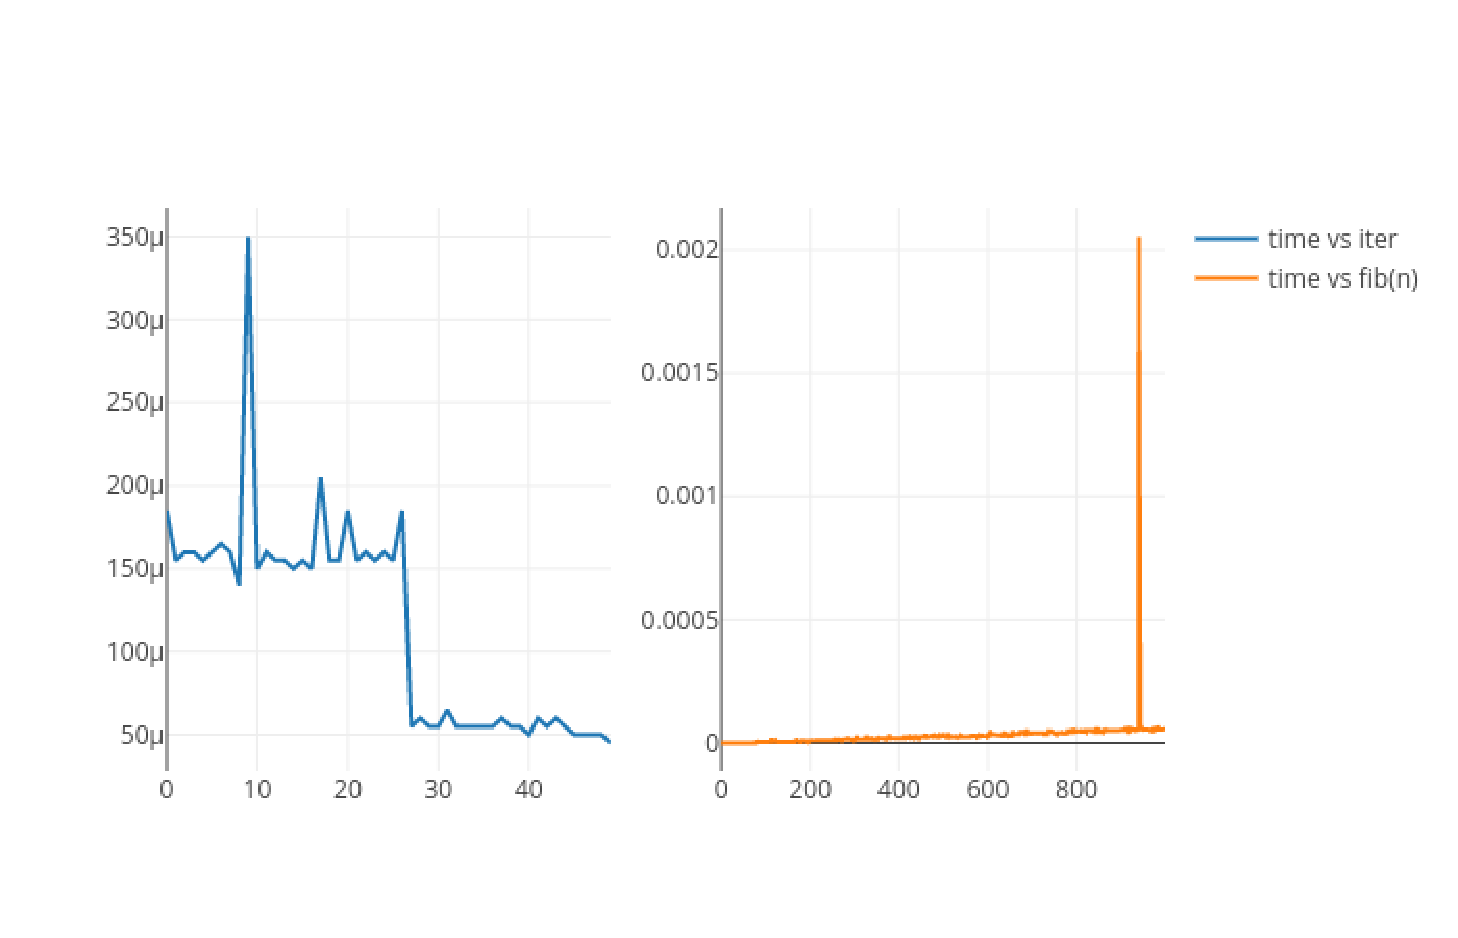
\includegraphics[width=\columnwidth]{figs/newplot15.pdf}
      \subcaption{}
    \end{minipage}
    \begin{minipage}{0.23\columnwidth}   
      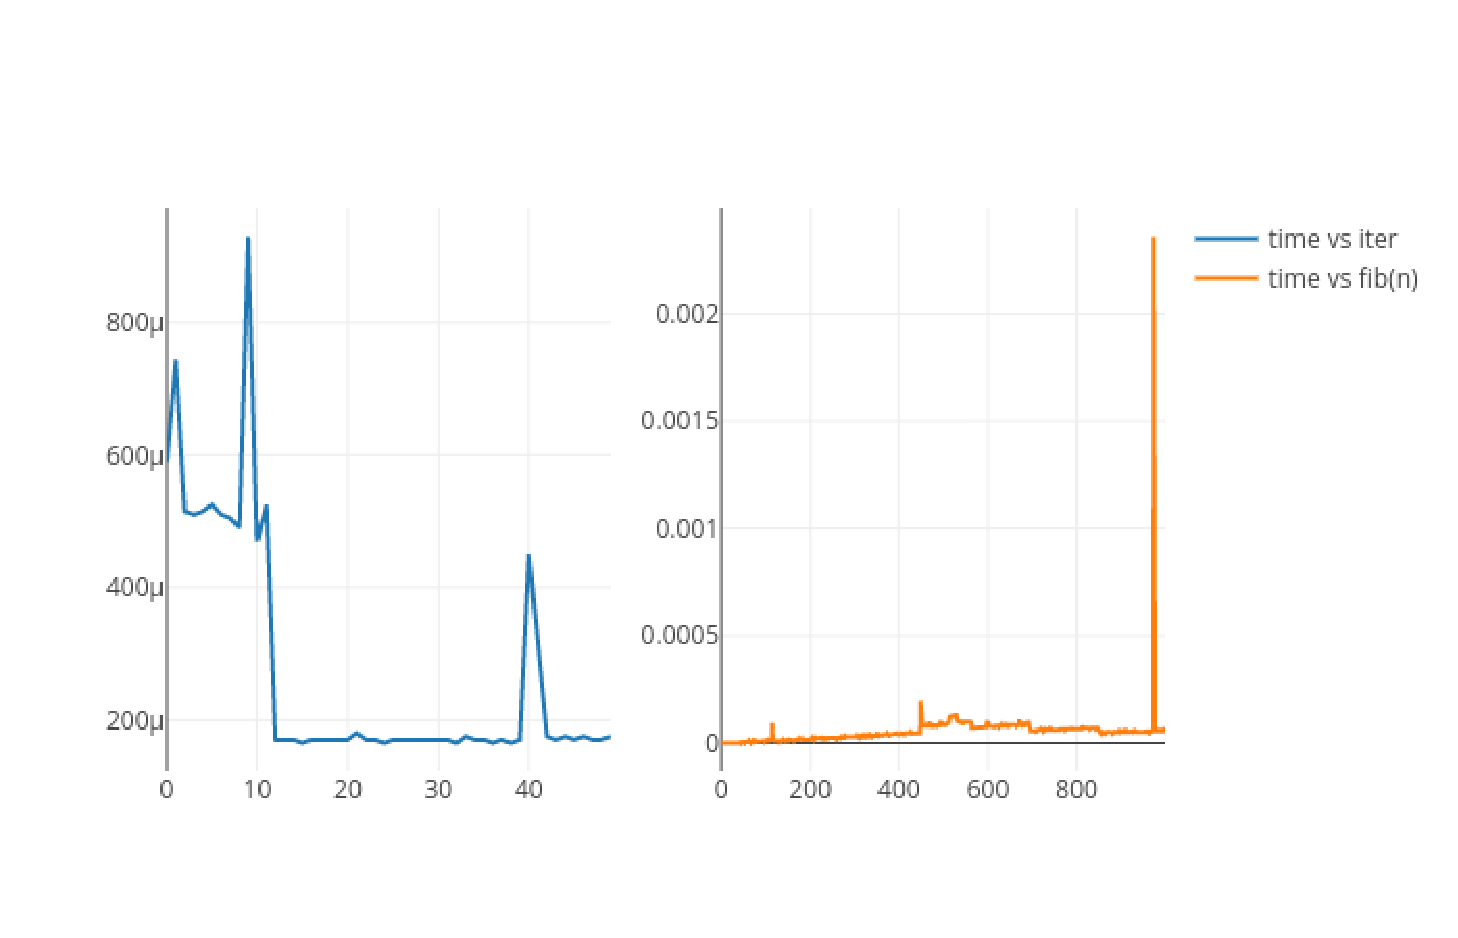
\includegraphics[width=\columnwidth]{figs/newplot16.pdf}
      \subcaption{}
    \end{minipage}
  \end{center}
  \caption{16回実験を行った結果}
  \label{figure:16}
\end{figure}


\bibliographystyle{junsrt}
\bibliography{p-report}

\end{document}
